%Appendix_A

%\appendixnodots   %this command is needed here, do not remove it

%%%%%%%%%%%%%%%%%%%%%%%%%%%%%%%%%%%%%%%%%%%%%%%%%%%%%%%%%%%%%%%%%%%%%%%%%%%%%%%%%%%%%%%%%%%%%%%%%%%
%%% Note: Name your appendix A, or B, or C, etc., but don't name it "APPENDIX A", etc. as the word
%%% APPENDIX will be automatically added in the name of the appendix in the text but it won't be
%%% added in the Table of Contents where it will appear only as A, B, C, etc., followed by the title.
%%% This is per new Grad School regulation as of January 2002.
\appendname{Appendix B: \\ \bigskip DASP Device Images}  
\appendix
\label{appendix:DASP Image Appendix}                   

\begin{figure}[htp]
	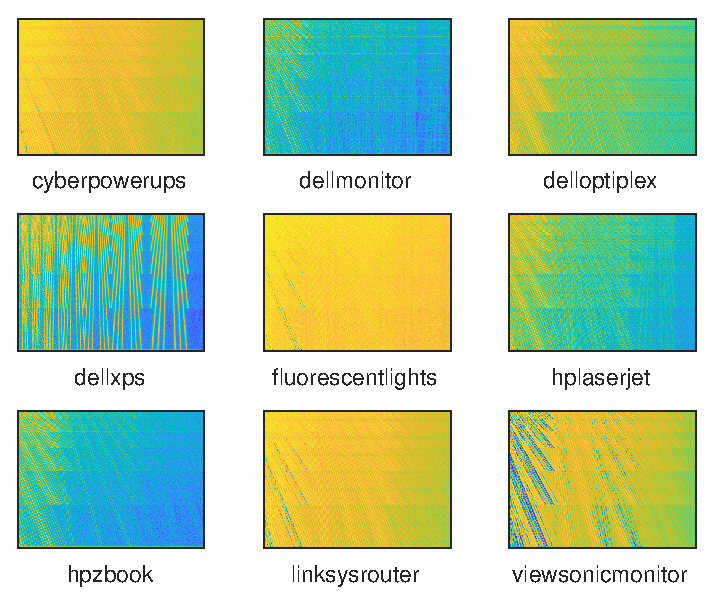
\includegraphics[width=0.75\textwidth]{./dasp_algorithm_results/dasp_device_images_cmasp_array.eps}
	\centering
	\caption{CMASP Array images of all test devices.}
	\label{fig:dasp_device_image_cmasp_array}
\end{figure}

\begin{figure}[htp]
	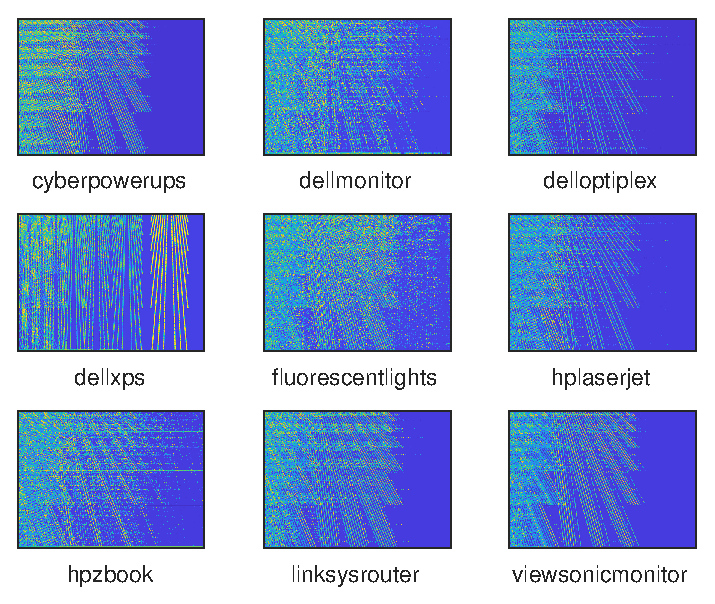
\includegraphics[width=0.75\textwidth]{./dasp_algorithm_results/dasp_device_images_cmasp_edgearray.eps}
	\centering
	\caption{CMASP Edge Array images of all test devices.}
	\label{fig:dasp_device_image_cmasp_earray}
\end{figure}
